\documentclass[UTF8]{article}
\usepackage{graphicx} % Required for inserting images
\usepackage{amsmath}
\usepackage{physics}
\usepackage{tcolorbox}
\usepackage{ctex}
\usepackage{tikz}
\usepackage{bookmark}
\usepackage[a4paper, top=2cm, bottom=2cm]{geometry}
\usepackage{esint}
\usepackage{booktabs}
% \usepackage{newtxmath}
\usepackage{times}
\usepackage{lmodern}



\title{一些重要的题目}
\author{}
\date{}

\begin{document}
\maketitle
\section{量子力学}
一个求矩阵元的小技巧:
\begin{align*}
    \begin{aligned}
         & \left\langle m\left|a x^3+b x^4\right| n\right\rangle=\left\langle m\left|a x^2 \cdot x\right| n\right\rangle+\left\langle m\left|b x^2 \cdot x^2\right| n\right\rangle \\
         & x=\sqrt{\frac{\hbar}{2 u w}}\left(a^{+}+a\right\rangle                                                                                                                  \\
         & x|n\rangle=\sqrt{\frac{\hbar}{2 u w}}(\sqrt{n}|n-1\rangle+\sqrt{n+1}|n+1\rangle)                                                                                        \\
         & \begin{aligned}
               x^2|n\rangle & =\frac{\hbar}{2 u w}\left(a^2+\left(a^{+}\right)^2+a a^{+}+a^{+} a\right)|n\rangle \\              
               & =\frac{\hbar}{2 u w}(\sqrt{n(n-1)}\ket{n-2}+(2n+1)\ket{n}
               +\sqrt{(n+1)(n+2)}\ket{n+2})
           \end{aligned}
    \end{aligned}
\end{align*}
\section{普物}
\subsection{振动}
对于质量为m的物体在斜面上的振动问题,容易搞混乱的就是如何建立坐标系,以及怎么在坐标系
中表示这个振动的过程。
\begin{figure}[htbp]
    \centering

    \tikzset{every picture/.style={line width=0.75pt}} %set default line width to 0.75pt        

    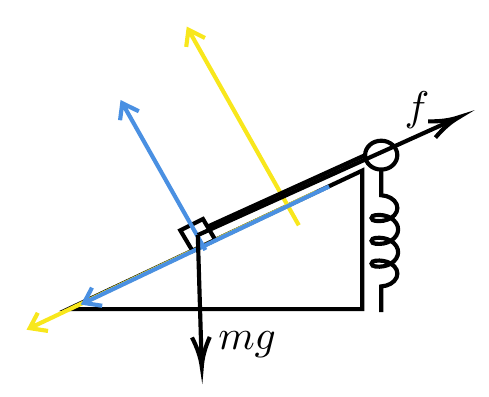
\begin{tikzpicture}[x=0.75pt,y=0.75pt,yscale=-1,xscale=1]
        %uncomment if require: \path (0,300); %set diagram left start at 0, and has height of 300

        %Shape: Right Triangle [id:dp695650597485965] 
        \draw  [line width=1.5]  (389.92,133.09) -- (248.22,199.83) -- (389.92,199.83) -- cycle ;
        %Shape: Axis 2D [id:dp550841046105645] 
        \draw [color={rgb, 255:red, 248; green, 231; blue, 28 }  ,draw opacity=1 ][line width=1.5]  (367.8,143.47) -- (229.69,208.99)(306.14,65.24) -- (359.31,159.44) (233.55,201.62) -- (229.69,208.99) -- (238.48,210.35) (314.11,69.2) -- (306.14,65.24) -- (305.07,73.49)  ;
        %Shape: Inductor (Air Core) [id:dp6688000653587656] 
        \draw  [line width=1.5]  (399.02,132.61) -- (399.02,144.97) .. controls (402.46,145.14) and (405.4,146.86) .. (406.43,149.29) .. controls (407.46,151.71) and (406.36,154.36) .. (403.67,155.95) .. controls (401.58,157.18) and (398.86,157.68) .. (396.23,157.32) .. controls (395.2,157.32) and (394.37,156.71) .. (394.37,155.95) .. controls (394.37,155.19) and (395.2,154.58) .. (396.23,154.58) .. controls (398.86,154.22) and (401.58,154.72) .. (403.67,155.95) .. controls (405.91,157.38) and (407.18,159.36) .. (407.18,161.44) .. controls (407.18,163.52) and (405.91,165.51) .. (403.67,166.93) .. controls (401.58,168.16) and (398.86,168.66) .. (396.23,168.31) .. controls (395.2,168.31) and (394.37,167.69) .. (394.37,166.93) .. controls (394.37,166.18) and (395.2,165.56) .. (396.23,165.56) .. controls (398.86,165.21) and (401.58,165.71) .. (403.67,166.93) .. controls (405.91,168.36) and (407.18,170.35) .. (407.18,172.42) .. controls (407.18,174.5) and (405.91,176.49) .. (403.67,177.92) .. controls (401.58,179.14) and (398.86,179.64) .. (396.23,179.29) .. controls (395.2,179.29) and (394.37,178.67) .. (394.37,177.92) .. controls (394.37,177.16) and (395.2,176.54) .. (396.23,176.54) .. controls (398.86,176.19) and (401.58,176.69) .. (403.67,177.92) .. controls (406.36,179.51) and (407.46,182.15) .. (406.43,184.58) .. controls (405.4,187.01) and (402.46,188.72) .. (399.02,188.9) -- (399.02,201.26) ;
        %Flowchart: Connector [id:dp7790313816423897] 
        \draw  [line width=1.5]  (391.26,125.66) .. controls (391.26,121.82) and (394.74,118.7) .. (399.02,118.7) .. controls (403.31,118.7) and (406.78,121.82) .. (406.78,125.66) .. controls (406.78,129.5) and (403.31,132.61) .. (399.02,132.61) .. controls (394.74,132.61) and (391.26,129.5) .. (391.26,125.66) -- cycle ;
        %Straight Lines [id:da8930630128726582] 
        \draw [line width=1.5]    (391.26,125.66) -- (315.82,159.9) ;
        %Shape: Rectangle [id:dp037257810343286124] 
        \draw  [line width=1.5]  (302.23,161.88) -- (313.15,156.45) -- (319.07,166.46) -- (308.16,171.89) -- cycle ;
        %Shape: Axis 2D [id:dp4887414649276913] 
        \draw [color={rgb, 255:red, 74; green, 144; blue, 226 }  ,draw opacity=1 ][line width=1.5]  (373.9,140.74) -- (255.81,196.87)(274.26,100.58) -- (314.3,171.39) (259.67,189.5) -- (255.81,196.87) -- (264.6,198.23) (282.23,104.54) -- (274.26,100.58) -- (273.2,108.83)  ;
        %Straight Lines [id:da6791031180439018] 
        \draw [line width=1.5]    (310.65,164.17) -- (312.48,224.58) ;
        \draw [shift={(312.57,227.58)}, rotate = 268.27] [color={rgb, 255:red, 0; green, 0; blue, 0 }  ][line width=1.5]    (14.21,-4.28) .. controls (9.04,-1.82) and (4.3,-0.39) .. (0,0) .. controls (4.3,0.39) and (9.04,1.82) .. (14.21,4.28)   ;
        %Straight Lines [id:da9763609362802905] 
        \draw [line width=1.5]    (310.65,164.17) -- (433.6,108.67) ;
        \draw [shift={(436.33,107.44)}, rotate = 155.71] [color={rgb, 255:red, 0; green, 0; blue, 0 }  ][line width=1.5]    (14.21,-4.28) .. controls (9.04,-1.82) and (4.3,-0.39) .. (0,0) .. controls (4.3,0.39) and (9.04,1.82) .. (14.21,4.28)   ;


        % Text Node
        \draw (408.35,93.3) node [anchor=north west][inner sep=0.75pt]  [font=\normalsize,xscale=1.5,yscale=1.5]  {$f$};
        % Text Node
        \draw (318.63,208.64) node [anchor=north west][inner sep=0.75pt]  [font=\normalsize,xscale=1.5,yscale=1.5]  {$mg$};


    \end{tikzpicture}
\end{figure}

\noindent 以黄色坐标轴建立坐标系,则:
\begin{gather*}
    mg\sin \theta - kx = m\frac{d^2(x-x_0)}{dt^2}\\
    kx_0-kx = -m\frac{d^2(x-x_0)}{dt^2}\\
    -ky=m\frac{d^2 y}{dt^2} \Longrightarrow y=y_m cos(\omega t + \varphi)
\end{gather*}
或者以平衡位置为原点建立坐标系:
\begin{gather*}
    mg\sin\theta -k(x+l_0) =m \frac{d^2x}{dt^2}\\
    -kx = m\frac{d^2 x}{dt^2}  \Longrightarrow x=x_m \cos (\omega t+\varphi)
\end{gather*}
一般情况下,我们使用平衡位置作为坐标系原点。
\subsection{波}
例子:波上的一点向下振动然后回到原点,所用的时间是多少,我的刻板影响就是$(\frac{\pi}{2}-\theta+\frac{\pi}{2})$,
但是这样其实

对于波向左传播还是向右传播所涉及到的相位的不同的分析,这里还是给出向左和向右
传播的波动方程:
\begin{align*}
    y = A \cos (\omega t- kx)\\
    y = A\cos (\omega t +k x)
\end{align*}
分析:如果是振动方程,第一个方程表示在x处的振动方程,$x=0$表示在原点的振动方程
,这个方程的物理意义就是,$x$处振动的方程的相位比波源处振动方程的相位落后$kx$;
如果是向左传播,如果左边的坐标都是小于0的,那物理意义和向右传播一样,都是相位
落后于波源的现象。

如果是波动方程,则第一个方程表示$t$时刻时的波形图,$t=0$表示此时的波形图,第一个方程
的物理意义就是$t$时刻处的波形的相位落后于$t=0$时刻的波形的相位$\omega t$。对于向左传播
的波形图也是类似分析。
\subsection{多普勒效应的分析}

\end{document}